% This is samplepaper.tex, a sample chapter demonstrating the
% LLNCS macro package for Springer Computer Science proceedings;
% Version 2.21 of 2022/01/12
%
\documentclass[runningheads]{llncs}
%
\usepackage[T1]{fontenc}
% T1 fonts will be used to generate the final print and online PDFs,
% so please use T1 fonts in your manuscript whenever possible.
% Other font encondings may result in incorrect characters.
%
\usepackage{graphicx}
% Used for displaying a sample figure. If possible, figure files should
% be included in EPS format.
%
% If you use the hyperref package, please uncomment the following two lines
% to display URLs in blue roman font according to Springer's eBook style:
%\usepackage{color}
%\renewcommand\UrlFont{\color{blue}\rmfamily}
%\urlstyle{rm}
%
\usepackage{listings}
\usepackage{xcolor} % Para poder usar colores
\usepackage{pdfpages}
\usepackage{hyperref}

\lstset{
    language=HTML,
    basicstyle=\ttfamily\small,      % Fuente monoespaciada
    keywordstyle=\color{blue},       % Etiquetas en azul
    stringstyle=\color{orange},      % Texto entre comillas en naranja
    commentstyle=\color{gray},       % Comentarios en gris
    breaklines=true,                 % Ajustar líneas largas
    frame=single,                    % Pone el recuadro (cuadrado)
    numbers=left,                    % Números de línea a la izquierda
    numberstyle=\tiny\color{gray},   % Estilo de los números
    showstringspaces=false,          % No mostrar espacios marcados
}
\begin{document}
%
\title{Módulo 1: Avogadro Toast}
%
%\titlerunning{Abbreviated paper title}
% If the paper title is too long for the running head, you can set
% an abbreviated paper title here
%
\author{Dinnocenzo Caterina \and
Kemelmajer Sara \and
Mujica Pilar\and
Martinez Rocio\and
Salamone Lucia\and
Segura Lucas}
%
\authorrunning{L. Salamone}
% First names are abbreviated in the running head.
% If there are more than two authors, 'et al.' is used.
%
\institute{Universidad Nacional de Cuyo, Instituto de Ingenería Industrial POBOX 5502 %\and
%Springer Heidelberg, Tiergartenstr. 17, 69121 Heidelberg, Germany
\email{luchisalamone10@gmail.com}\\
\url{https://ingenieria.uncuyo.edu.ar/}} %\and
%ABC Institute, Rupert-Karls-University Heidelberg, Heidelberg, Germany\\
%\email{\{abc,lncs\}@uni-heidelberg.de}}
%
\maketitle              % typeset the header of the contribution
%
\begin{abstract}
Durante el Módulo 1 adquirimos las bases fundamentales para el trabajo colaborativo y la creación de contenidos digitales orientados a proyectos académicos y profesionales. En la primera clase comenzamos creando nuestras cuentas en GitHub,\cite{githubdocs} donde configuramos un repositorio personal y también un repositorio grupal. Organizamos los equipos de trabajo, definimos un nombre e identidad (incluyendo logo) y aprendimos a estructurar información mediante tablas e inserción de imágenes, además de crear páginas individuales en Markdown y vincularlas a la página del grupo.

En la segunda clase incorporamos herramientas complementarias como Google Colab, lo \cite{lopez2003latex} que nos permitió familiarizarnos con notebooks. También aprendimos a crear archivos HTML de forma manual y exploramos conceptos básicos de HTML siguiendo estándares W3C, aplicándolos en la construcción de una landing page simple.

En la tercera clase dimos \cite{sepulcre2024uso} el salto a la escritura académica con LaTeX mediante Overleaf. Creamos nuestras cuentas, exploramos su funcionamiento y seleccionamos plantillas. A partir de esto, comenzamos el desarrollo de nuestro currículum en LaTeX, enfocándonos en la estructura profesional y presentación formal.

En conjunto, el módulo nos brindó herramientas clave para el trabajo en equipo, el manejo de repositorios \cite{loeliger2012version} y la generación de contenido técnico estructurado.


\keywords{UNCuyo \and TyHM \and markuo language.}
\end{abstract}
%
%
%
\section{Introducción}
Tras haber consolidado las bases del trabajo colaborativo y la gestión de repositorios, este informe se centra en la aplicación técnica de los lenguajes de marcado aprendidos. A continuación, se presenta una demostración práctica de la implementación de etiquetas HTML para la estructuración de contenidos web. Asimismo, se detalla el uso de Markdown como herramienta de documentación rápida y se expone la transición hacia la escritura académica formal mediante el uso de la plantilla oficial de \cite{colabgithub}Springer en LaTeX. Finalmente, se incluye una síntesis comparativa de las competencias adquiridas y la integración del currículum profesional dentro de este mismo documento.

\section{Uso básico del lenguaje HTML}

\begin{lstlisting}[language=HTML]
<html>
<head>
<title>Mi primera pagina</title>
</head>
<body>
<h1>Mi primera página web</h1>
Esto es el cuerpo del texto.
<p>Esto es un parrafo</p>
<ul>
<li>Primero</li>
<li>Segundo</li>
<li>Tercero</li>
</ul>
</body>
</html>
\end{lstlisting}

\section{Lenguajes de Marcado: Markdown y LaTeX}

Además de HTML, en este módulo aplicamos otros lenguajes de marcado esenciales para la documentación técnica y académica:

\subsection{Markdown en GitHub}
Markdown permite dar formato de manera rápida y sencilla, ideal para archivos \texttt{README.md} en repositorios. A continuación, se muestra un ejemplo de la sintaxis utilizada:

\begin{lstlisting}[caption=Ejemplo de sintaxis Markdown]
# Titulo del Proyecto
## Subtitulo de seccion
Este es un parrafo con texto en **negrita** e *italica*.
* Elemento de lista 1
* Elemento de lista 2
[Enlace al repositorio](https://github.com/tu-usuario/proyecto)
\end{lstlisting}

\subsection{Escritura Academica en LaTeX}
LaTeX es el estándar para la edición de documentos científicos. Su estructura se basa en comandos que definen la jerarquía del documento, como se observa en el siguiente fragmento:

\begin{lstlisting}[language=TeX, caption=Sintaxis basica de LaTeX]
\section{Introduccion}
\subsection{Subseccion}
Este es un texto con una cita bibliografica \cite{lopez2003latex}.
\begin{itemize}
    \item Primer punto de la lista.
    \item Segundo punto de la lista.
\end{itemize}
\end{lstlisting}

\section{Guías de Referencia (Cheatsheets)}

Para la correcta implementación de los lenguajes de marcado y el uso de las herramientas del módulo, se consultaron las siguientes guías rápidas y documentación oficial:

\begin{itemize}
    \item \textbf{Markdown:} \href{https://www.markdownguide.org/cheat-sheet/}{Markdown Guide Cheat Sheet}.
    \item \textbf{HTML5:} \href{https://www.w3schools.com/tags/default.asp}{W3Schools HTML Reference}.
    \item \textbf{LaTeX:} \href{https://overleaf.com/learn}{Overleaf Documentation and Wiki}.
    \item \textbf{Git \& GitHub:} \href{https://education.github.com/git-cheat-sheet-education.pdf}{GitHub Education Git Cheat Sheet}.
\end{itemize}

\section{Comparativa de Competencias Adquiridas}

A modo de síntesis, la Tabla~\ref{tab_comparativa} resume la evolución técnica experimentada durante el desarrollo de este primer módulo, comparando la metodología de trabajo previa con los estándares profesionales incorporados.

\begin{table}[h!]
\centering
\caption{Comparativa de situación antes y después del Módulo 1.}
\label{tab_comparativa}
\begin{tabular}{|l|p{4.5cm}|p{4.5cm}|}
\hline
\textbf{Área de Trabajo} & \textbf{Situación Inicial (Antes)} & \textbf{Situación Actual (Después)} \\ \hline
\textbf{Gestión de Archivos} & Uso de carpetas locales, envío de versiones por mail o Drive. & Repositorios centralizados en \textbf{GitHub} con control de versiones real. \\ \hline
\textbf{Edición de Texto} & Formato manual en Word (dependencia del mouse y menús). & Escritura técnica en \textbf{LaTeX} mediante comandos lógicos y estructura. \\ \hline
\textbf{Estructura Web} & Desconocimiento de la sintaxis y etiquetas del navegador. & Creación y comprensión de jerarquías con \textbf{HTML5} (W3C). \\ \hline
\textbf{Colaboración} & Edición lineal o sobreescritura de archivos compartidos. & Flujo de trabajo profesional en equipo (grupos de GitHub). \\ \hline
\end{tabular}
\end{table}

\section{Conclusión}
La experiencia en este primer módulo ha marcado un cambio en nuestra forma de producir contenido técnico. La principal ventaja que destaco es la capacidad de separar el contenido de la forma: mientras que en procesadores de texto tradicionales el formato suele ser un obstáculo, lenguajes como LaTeX y HTML permiten una estructura lógica y profesional desde el inicio.

Considero que estas técnicas serán fundamentales en mi futuro académico y profesional, especialmente para la redacción de informes de ingeniería, proyectos de investigación y el futuro proyecto final de grado, donde la precisión técnica y el cumplimiento de normativas editoriales son críticos. La integración de GitHub como soporte para el control de versiones garantiza, además, que el trabajo sea recuperable y colaborativo, una habilidad indispensable en cualquier entorno laboral moderno.

\section{Anexos}

\subsection{Currículum Vitae}
A continuación, se adjunta el currículum vitae profesional como parte de la documentación integral de este módulo, demostrando la aplicación práctica de los estilos de edición aprendidos.

% Este comando mete el PDF en hojas nuevas automáticamente
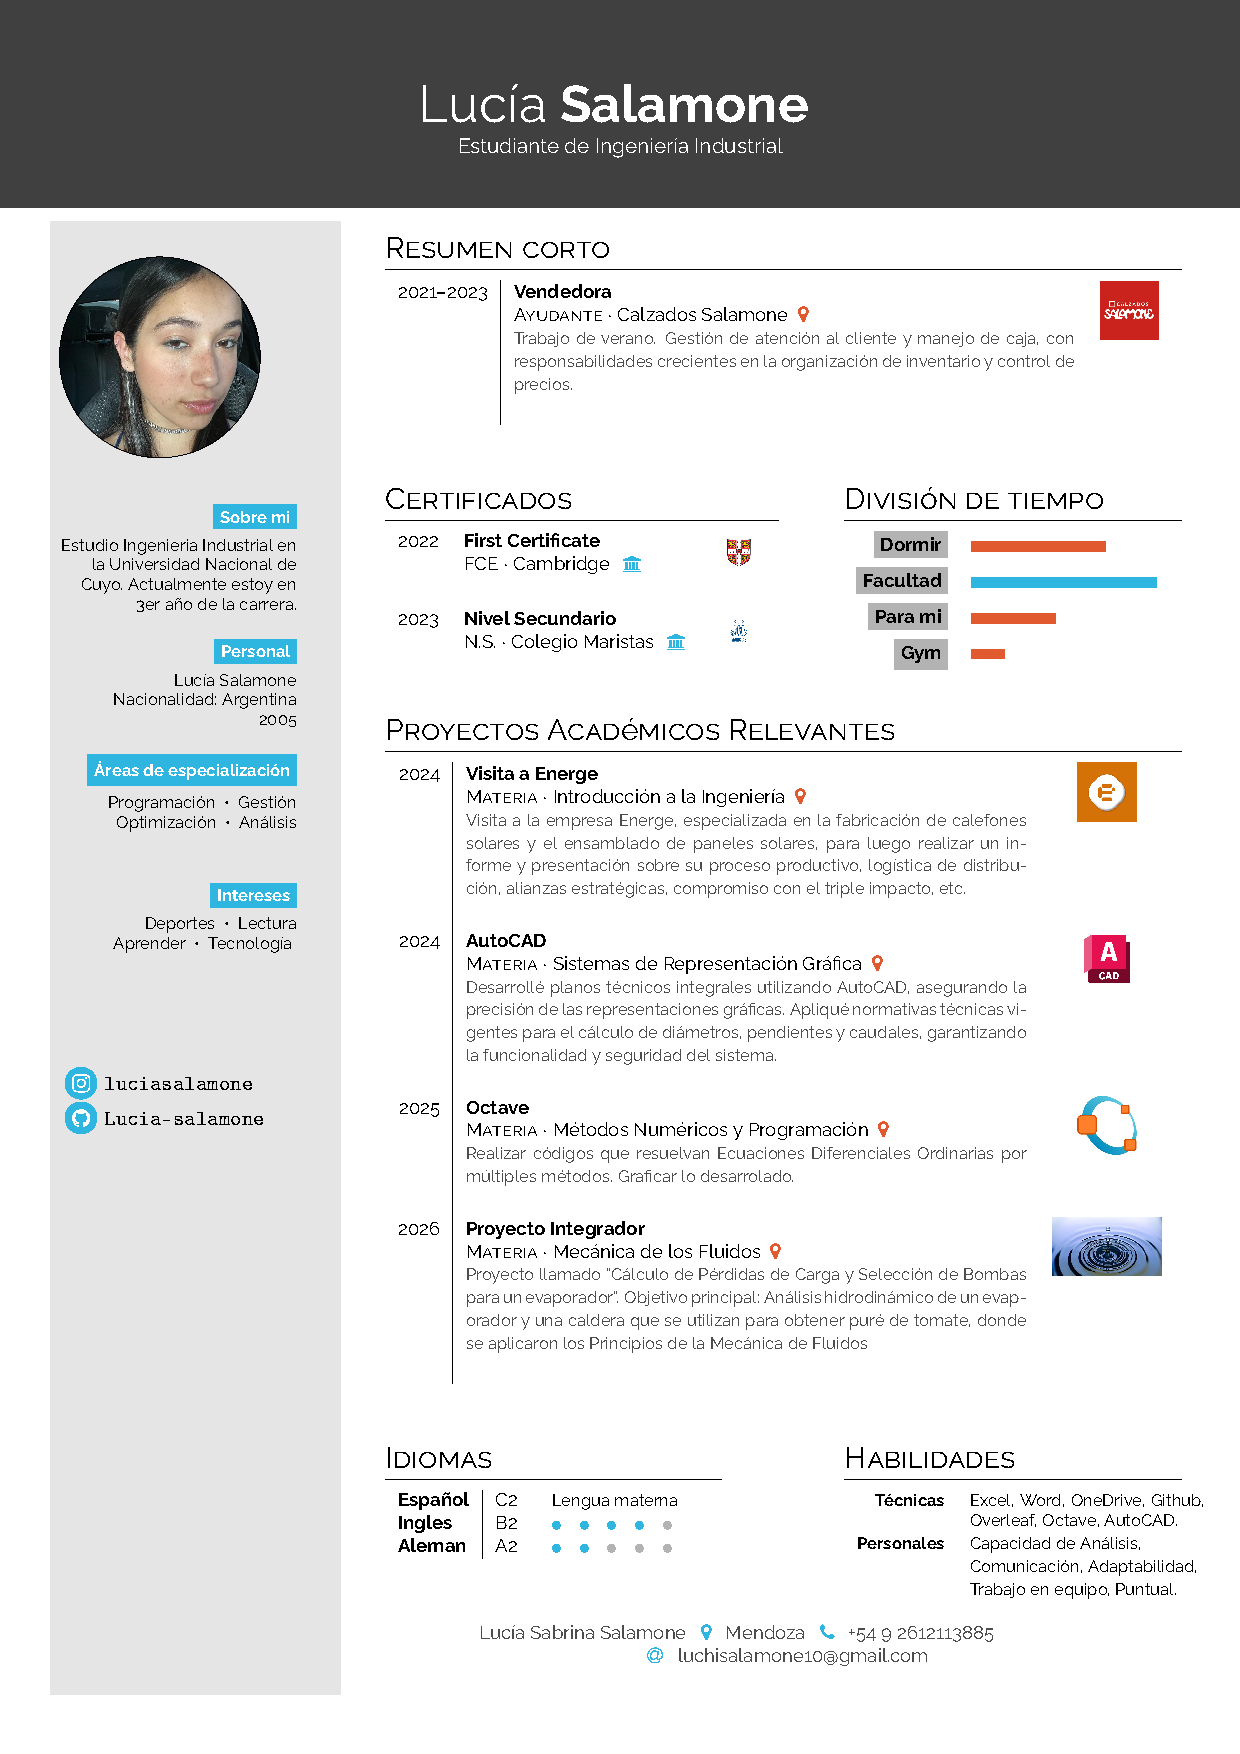
\includepdf[pages=-, pagecommand={\thispagestyle{plain}}]{CV_Lucia_Salamone.pdf}

%
% ---- Bibliography ----
%
% BibTeX users should specify bibliography style 'splncs04'.
% References will then be sorted and formatted in the correct style.
%
% \bibliographystyle{splncs04}
% \bibliography{mybibliography}
%
\bibliographystyle{splncs04} 
\bibliography{bibliografia} % <-- Aquí pones el nombre exacto de tu archivo sin el .bib
\end{document}